% SHORT SPEAKER EXPLAINER for the visual-first review poster (poster_visual_final_review.pdf), 19 October 2026.
% REVIEW DRAFT for Toni, Chris and Pierce. Every number: records/CORA_SUMMIT_CLAIM_LEDGER_20261017.md (audited in
% POSTER_CLAIM_AUDIT.md). Figures: figures/ (scripts/summit_visual_figures.py; provenance in POSTER_FIGURE_PROVENANCE.json).
% The earlier explainer_review.tex and docs/summit_poster/explainer.tex are preserved unchanged.
\documentclass[11pt]{article}
\usepackage[a4paper, margin=2.2cm]{geometry}
\usepackage[scaled]{helvet}
\renewcommand{\familydefault}{\sfdefault}
\usepackage[T1]{fontenc}
\usepackage{microtype}
\usepackage{xcolor}
\usepackage{enumitem}
\usepackage{booktabs}
\usepackage{array}
\usepackage{graphicx}
\usepackage{needspace}
\usepackage{tikz}
\usetikzlibrary{positioning, arrows.meta}
\definecolor{ink2}{HTML}{52514E}
\definecolor{accent}{HTML}{2A78D6}
\definecolor{critical}{HTML}{D03B3B}
\pagestyle{plain}
\pdftrailerid{}
\setlength{\parindent}{0pt}
\setlength{\parskip}{0.45em}
\setlist{itemsep=0.1em, topsep=0.15em, parsep=0pt}
\raggedright
\newcommand{\cue}[1]{{\color{ink2}\textit{[#1]}}\par}
\newcommand{\page}[1]{\clearpage{\Large\bfseries #1}\par\vspace{0.2em}}
\newcommand{\sub}[1]{\par\needspace{6\baselineskip}\vspace{0.5em}{\large\bfseries\color{accent}#1}\par}
\newcommand{\term}[1]{\textbf{#1}}
\tikzset{stage/.style={rounded corners=4pt, draw=accent, line width=1.2pt, fill=white, align=center,
         font=\small, text width=3.6cm, inner sep=4pt},
         pstage/.style={stage, dashed, draw=ink2},
         flow/.style={-{Latex[length=2.5mm]}, line width=1pt, draw=ink2}}

\begin{document}
{\LARGE\bfseries Learning What to Change: the poster, explained\par}
\vspace{0.2em}
{\color{ink2} Short speaker explainer for the visual-first review poster, 19 October 2026. REVIEW DRAFT for Toni,
Chris and Pierce before anything is printed.\par}
\begin{itemize}
  \item \textbf{How to use it.} Read the plain text aloud. Grey bracketed lines are notes to you.
  \item \textbf{Numbers.} Every number is in \texttt{records/CORA\_SUMMIT\_CLAIM\_LEDGER\_20261017.md}, with its
        scope, and is audited against the poster in \texttt{POSTER\_CLAIM\_AUDIT.md}.
  \item \textbf{Figures.} Real figures are drawn from hash-pinned recorded data. The one illustrative figure says so.
  \item \textbf{The longer research dossier.} A deeper companion is kept separate; it is not available on Athe for
        this session. This explainer relies only on the records named here.
\end{itemize}

\sub{The 20-second version}
I study how a reasoning system can tell what to change when its explanation of a problem is not good enough: the
objects it sees, the rule it uses, or simply the evidence it has. My system, CORA, solves ARC puzzles by writing small
programs. It once built a new rule on a real puzzle and checked it carefully. But a version that ignored its failure
record did the same, and on 58 more puzzles construction added nothing. Learning which change helps is the open
problem I am now testing.

\sub{The 90-second version}
\cue{full script, with pointing cues: POSTER\_90\_SECOND\_SCRIPT.md}
\begin{itemize}
  \item \textbf{The question.} When a reasoner's explanation is inadequate, can it work out whether it needs
        different objects, a different rule, or better evidence, and choose a change that improves predictions on new
        problems?
  \item \textbf{The test.} ARC gives two or three examples and a new input, so it is a clean place to test this.
  \item \textbf{Fitting is not explaining.} On 60 exposed training puzzles, CORA's checker accepted 6 answers, all
        correct. But on 26 puzzles every rule that fit the examples failed the test.
  \item \textbf{A rule CORA built.} On one real puzzle CORA built a new conditional rule: blue objects send a line
        up-left, red ones down-right. It rebuilt the rule three times with an example held out, and it was right.
  \item \textbf{The limit.} A version that ignored the failure record found the same rule, and on 58 further puzzles
        construction added zero verified solves.
  \item \textbf{Next.} CORA-v2 can already notice some inadequacy, such as competing hypotheses or an example the
        rule rests on alone. What is not yet shown is choosing the revision that helps.
\end{itemize}

\sub{The two-minute version}
Add to the 90-second version:
\begin{itemize}
  \item \textbf{Four reasons an explanation fails} (the illustrative panels): memorizing, wrong objects, a missing
        rule, too little evidence. A failing system does not know which one happened.
  \item \textbf{What the 0 of 58 suggests.} An evaluator-only check suggests most lie outside the single-rule language
        construction used: a hypothesis about expressivity, not proof of new semantics.
  \item \textbf{The neural baseline.} My reproduction of the third-party NVARC method scores 27.64; it is not CORA.
        Native CORA and CORA with rule construction score 0.00.
  \item \textbf{Biology.} What might transfer is the revision policy, not the grid operations: future work, untested.
\end{itemize}

%------------------------------------------------------------------------------------------------- page 2
\page{1. The question: why objects, rules, evidence and revision are different problems}
\cue{poster banner}
\textbf{The question, shaped in conversation with Toni Kazic:} can a system induce useful representations and
executable rules from a few observations, recognize when its explanation is inadequate, decide what must change, and
carry that way of revising into a domain whose meaning is different? These are research aims. CORA has not achieved
them all.

\textbf{Words used on the poster, and here.}
\begin{itemize}
  \item \term{Representation}: how a grid is broken into objects and parts.
  \item \term{Rule}: executable instructions that change the grid.
  \item \term{Grammar} or \term{rule language}: the set of rules a system can express at all.
  \item \term{Memorization}: copying apparent regularities in the examples without a relation that transfers.
  \item \term{Evidence gap}: the examples do not distinguish between plausible hypotheses.
  \item \term{Leave-one-out}: rebuild the rule with one example hidden, and check that it predicts that example.
  \item \term{Failure diagnosis}: identifying an \emph{observable} reason to doubt or revise the current explanation.
        It does not mean knowing that the hidden test answer is wrong; CORA never sees it.
  \item \term{Certified}: unique, and rebuilt in every leave-one-out check.
  \item \term{Exploratory}: executable and consistent with every example, but not certified. Never counted as a
        verified solve.
  \item \term{Generalization}: correct answers on new task instances, evaluated separately under a declared exposure
        boundary.
\end{itemize}

\textbf{Why the four are different problems.} The same failure, a wrong answer, can come from four places, and each
needs a different repair:
\begin{itemize}
  \item the \emph{objects} were wrong: revise the representation;
  \item the \emph{rule language} lacked the operation: extend the language;
  \item the examples did not \emph{decide}: keep alternatives, abstain, or ask for evidence;
  \item the rule was \emph{memorized}: a fit that does not transfer.
\end{itemize}
The wrong repair can break what already worked. For example, adding rules everywhere can turn a unique answer into a
tie (page 7). The research problem is to tell these apart from the examples alone, choose a repair, and show that the
choice beats doing everything blindly.

%------------------------------------------------------------------------------------------------- page 3
\page{2. What an ARC task is (poster column 1)}
\begin{minipage}[t]{0.52\linewidth}
\vspace{0pt}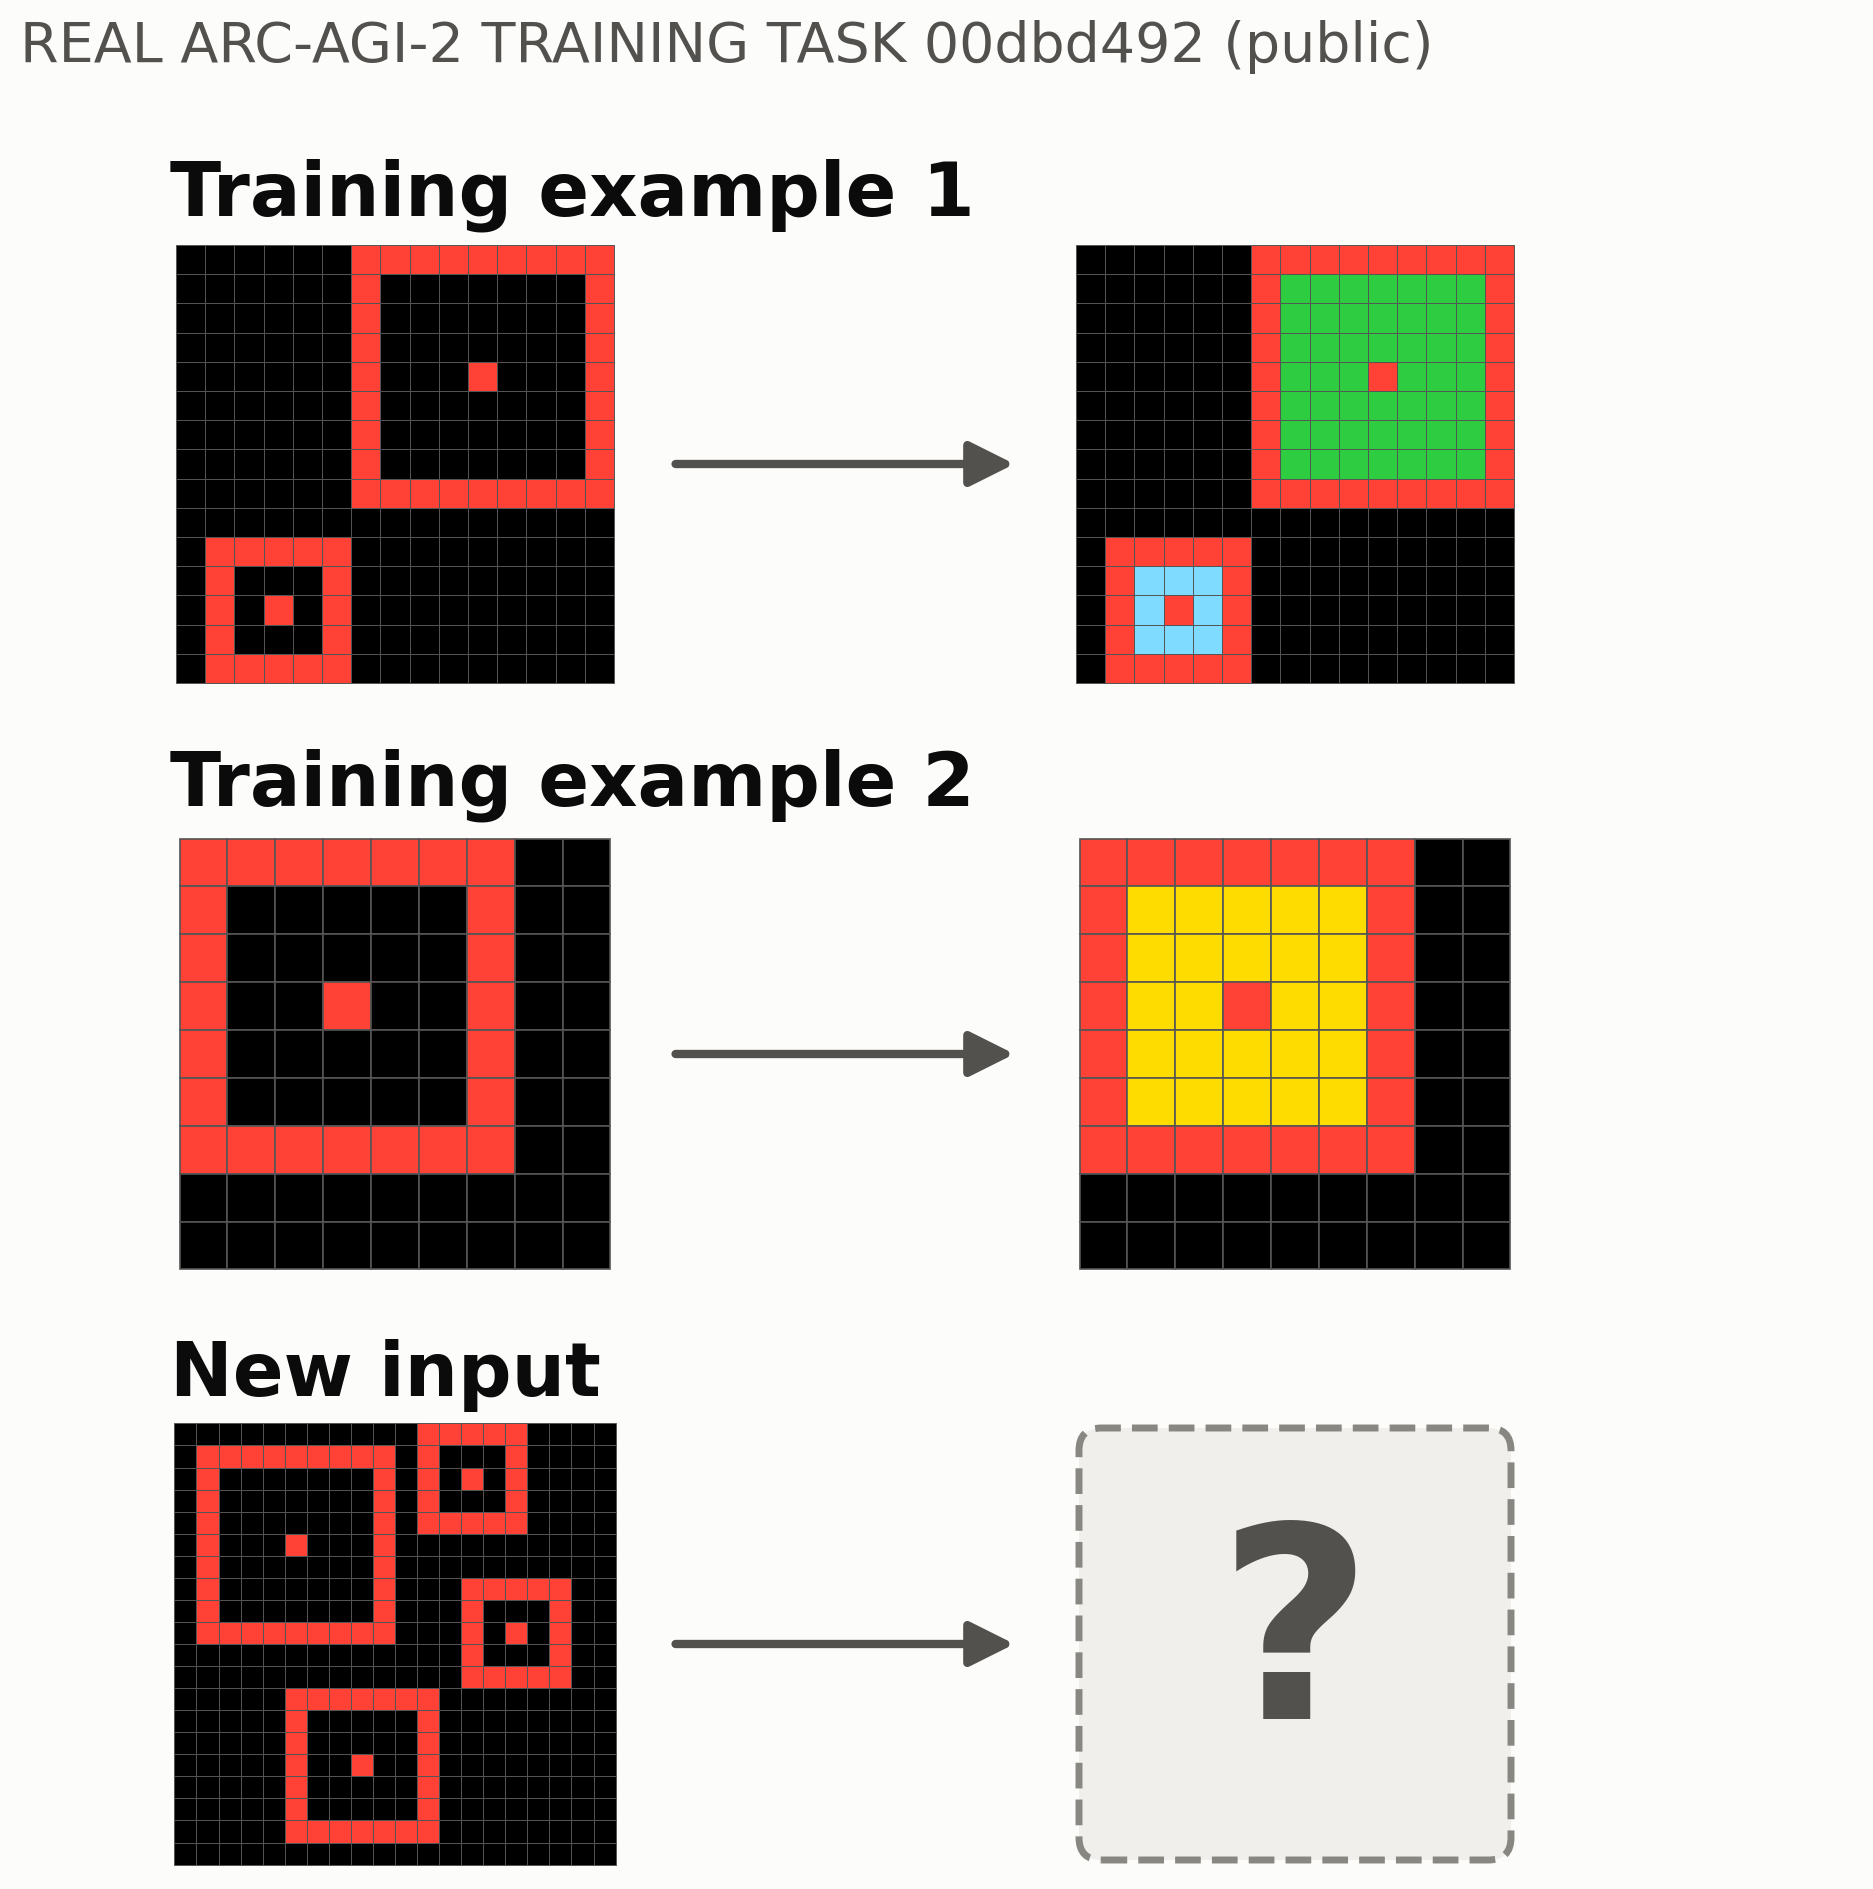
\includegraphics[width=\linewidth]{figures/fig_arc_intro_00dbd492.png}
\end{minipage}\hfill
\begin{minipage}[t]{0.44\linewidth}
\vspace{0pt}
\textbf{Figure: real task 00dbd492}, a public ARC-AGI-2 training task. Grids are drawn cell for cell from the
recorded bundle \texttt{v2\_witness\_00dbd492.json} (in \texttt{docs/summit\_demo\_20261023/data/}).
\begin{itemize}
  \item \textbf{Semantics.} A grid is a small array of colours 0--9 (0 is black). A task gives a few training pairs
        (input $\to$ output) and a new input.
  \item \textbf{The task.} The solver must produce the new output exactly, with two attempts allowed. Here each frame
        is filled with a colour set by its size.
  \item \textbf{Memorization versus generalization.} A rule like ``paint the cells that changed in example 1'' fits
        example 1 and fails elsewhere: that is memorization. ``Fill each frame with the colour its size calls for''
        generalizes.
  \item \textbf{Exposure.} This task was examined during CORA-v2 development; it is used here only to explain ARC.
\end{itemize}
\end{minipage}

\sub{The four illustrative panels}
\begin{minipage}[t]{0.52\linewidth}
\vspace{0pt}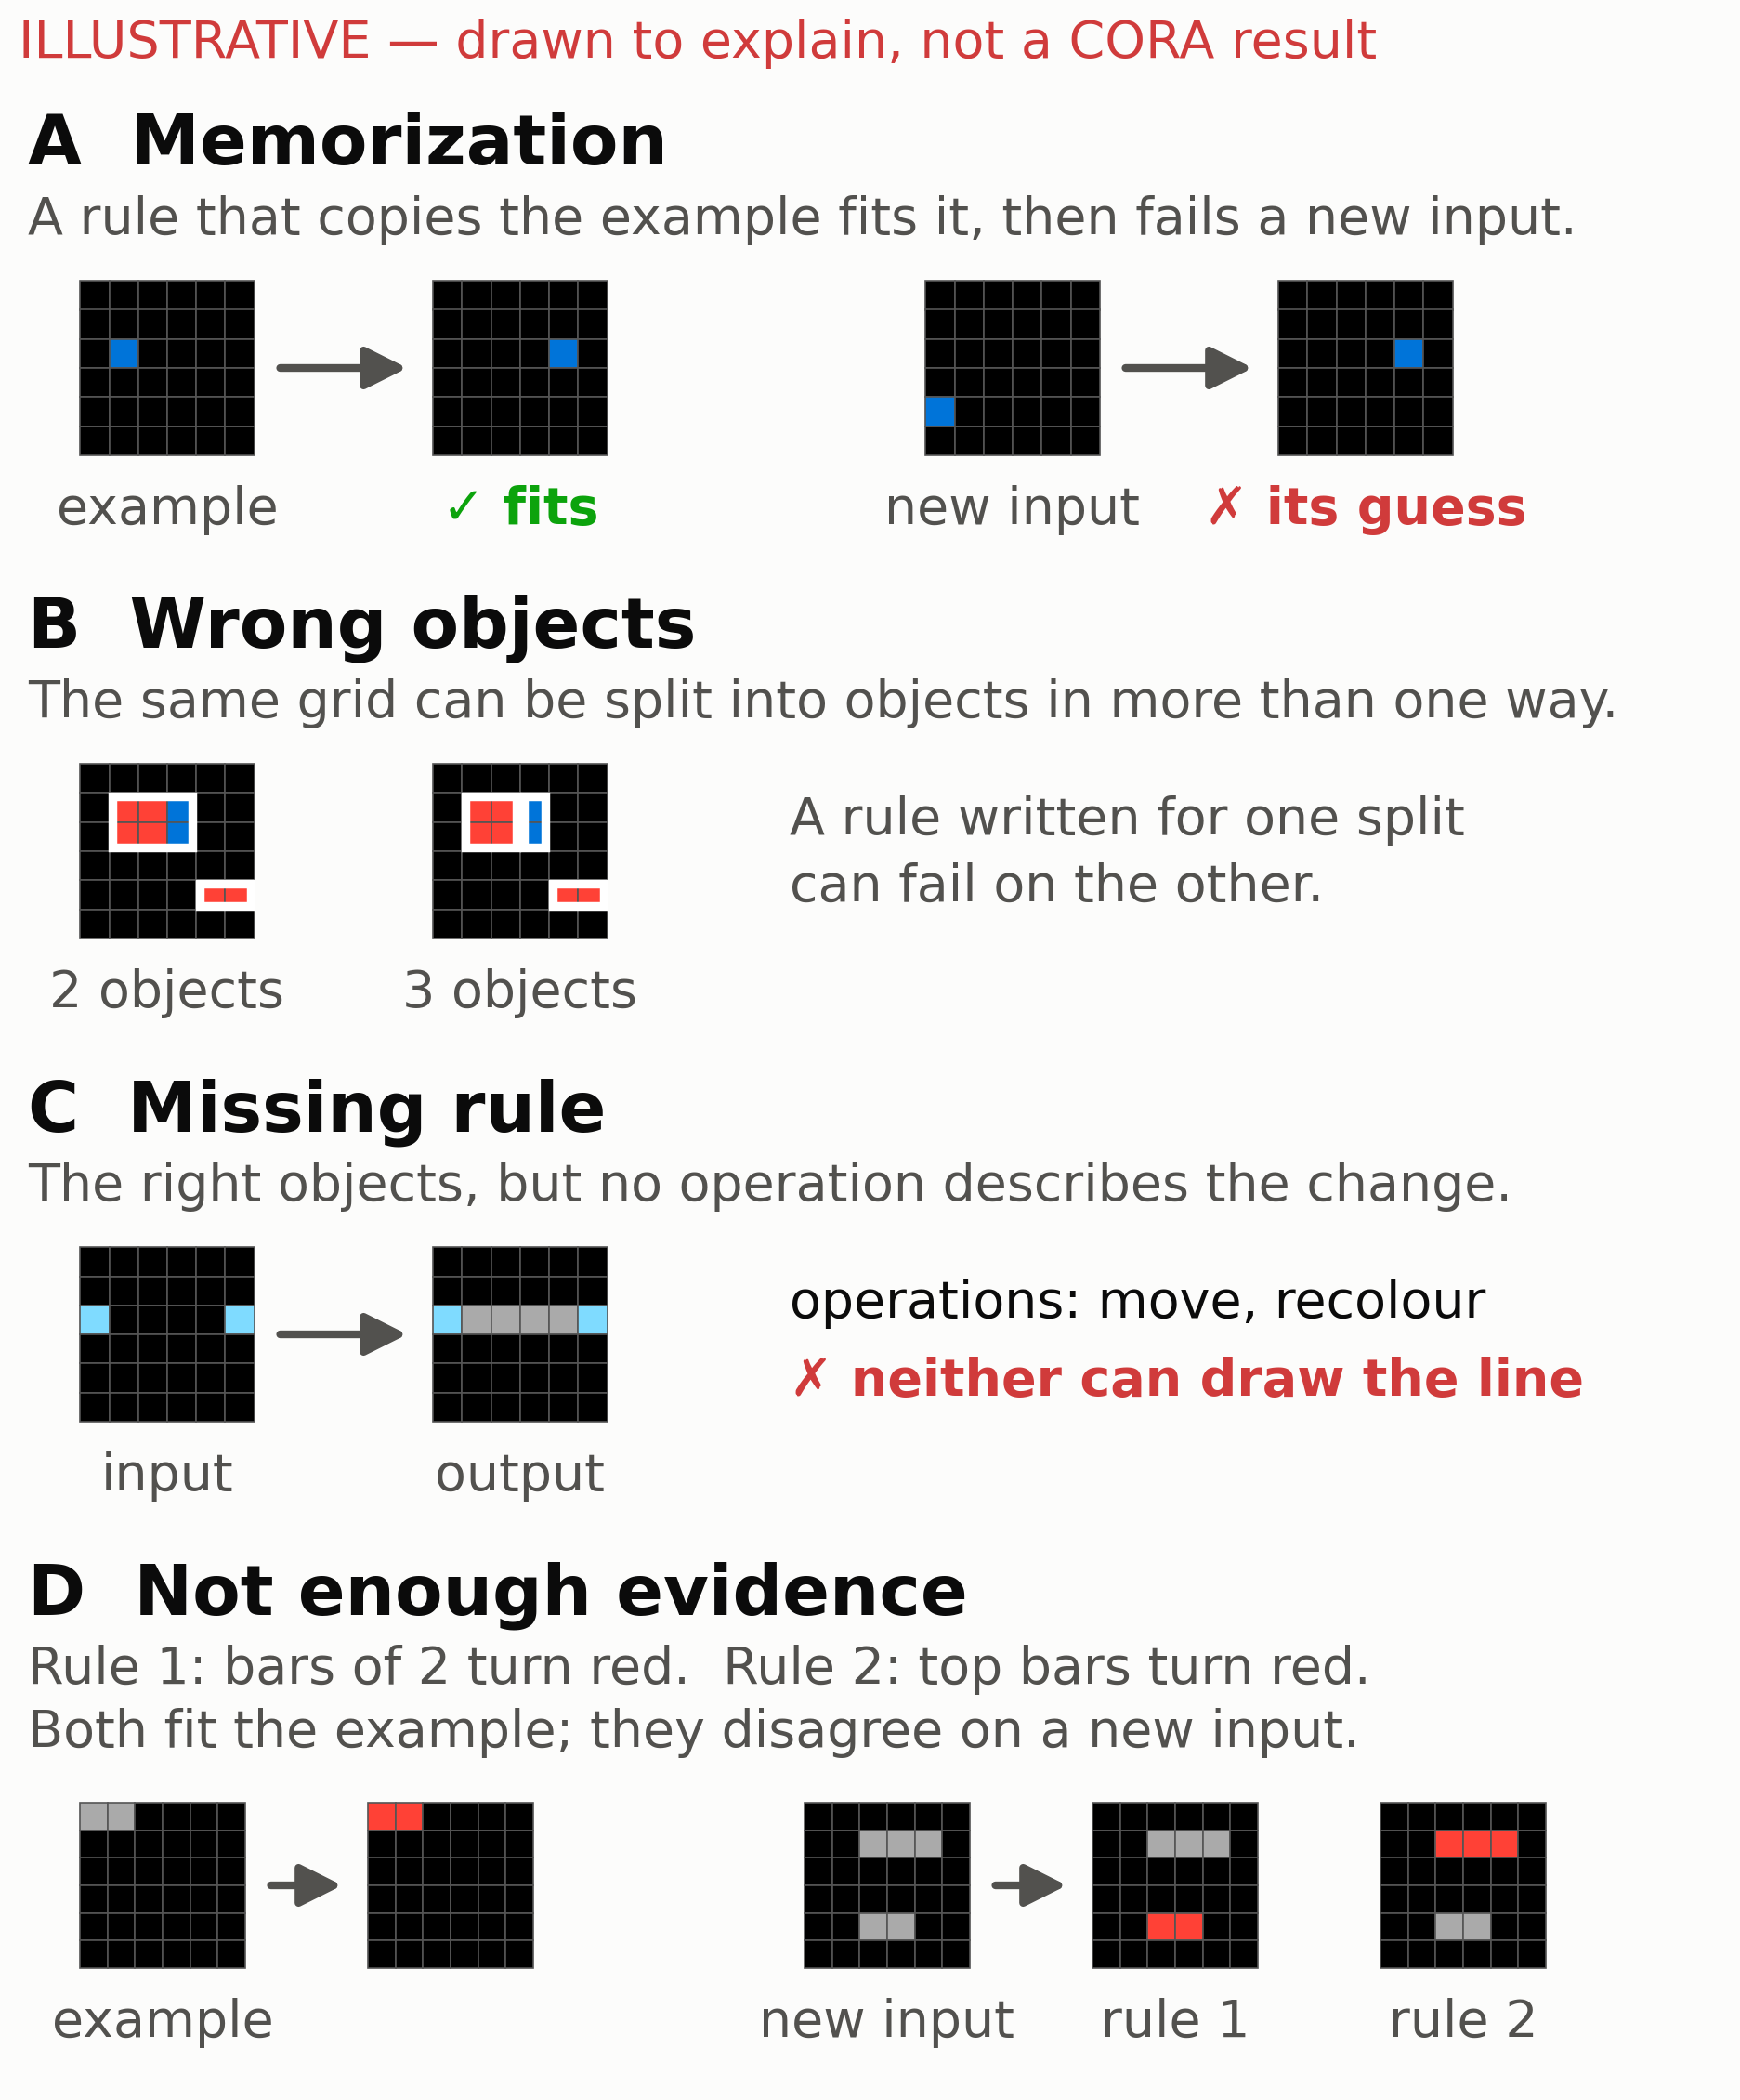
\includegraphics[width=\linewidth]{figures/fig_four_reasons_ILLUSTRATIVE.png}
\end{minipage}\hfill
\begin{minipage}[t]{0.44\linewidth}
\vspace{0pt}
\textbf{ILLUSTRATIVE}: drawn to explain, not an ARC task and not a CORA result.
\begin{itemize}
  \item \textbf{A.} A rule that copies the example's output fits it, then fails a new input.
  \item \textbf{B.} The same grid, split into 2 or 3 objects, depending on whether touching cells of different colours
        count as one object.
  \item \textbf{C.} The right objects, but the available operations (move, recolour) cannot draw the connecting line.
  \item \textbf{D.} ``Bars of 2 turn red'' and ``top bars turn red'' both fit the example and disagree on a new input.
\end{itemize}
\end{minipage}

%------------------------------------------------------------------------------------------------- page 4
\page{3. CORA today: what is built, and what is a goal}
\cue{poster column 2 (pipeline) and column 3 (loop)}
\begin{center}
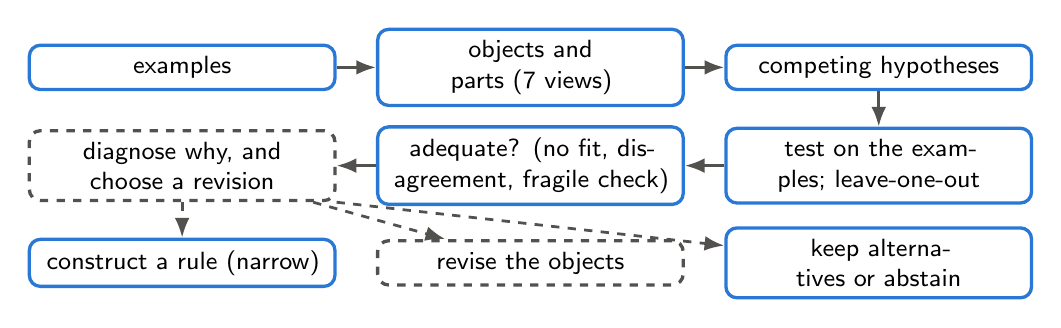
\begin{tikzpicture}[node distance=0.45cm and 0.5cm]
  \node[stage] (a) {examples};
  \node[stage, right=of a] (b) {objects and parts (7 views)};
  \node[stage, right=of b] (c) {competing hypotheses};
  \node[stage, below=of c] (d) {test on the examples; leave-one-out};
  \node[stage, left=of d] (e) {adequate? (no fit, disagreement, fragile check)};
  \node[pstage, left=of e] (f) {diagnose why, and choose a revision};
  \node[stage, below=of f] (g) {construct a rule (narrow)};
  \node[pstage, right=of g] (h) {revise the objects};
  \node[stage, right=of h] (i) {keep alternatives or abstain};
  \draw[flow] (a) -- (b); \draw[flow] (b) -- (c); \draw[flow] (c) -- (d); \draw[flow] (d) -- (e); \draw[flow] (e) -- (f);
  \draw[flow, dashed] (f) -- (g); \draw[flow, dashed] (f) -- (h); \draw[flow, dashed] (f.south east) -- (i);
\end{tikzpicture}
\end{center}
Solid outlines: implemented and tested. Dashed: proposed, or not yet validated.
\begin{itemize}
  \item \textbf{Native CORA (v23).} The frozen original system.
        \begin{itemize}
          \item It segments a grid into objects in seven ways (``views'').
          \item It searches for an object program that reproduces every example.
          \item It accepts only answers that survive leave-one-out rebuilding.
          \item Its whole harness adds other solver layers and gives two attempts.
        \end{itemize}
  \item \textbf{CORA-FHR} (failure-conditioned hypothesis revision), the rule-construction experiment.
        \begin{itemize}
          \item It reads native's own failure trace and constructs a missing growth operation from a typed grammar of
                37,750 expressions (G-grow).
          \item It installs the operation reversibly and accepts it only if the unchanged engine uses it and every
                fold rebuilds it.
          \item A \term{witness} is one recorded run that shows the whole chain end to end.
        \end{itemize}
  \item \textbf{CORA-v2}, the hypothesis reasoner.
        \begin{itemize}
          \item It keeps every hypothesis (representation, geometry, colour policy) that reproduces every example: its
                \term{version space}.
          \item It abstains when they disagree, and reruns the search with each example held out.
          \item It labels why it is unsure, with observable \emph{diagnoses}, and offers exploratory guesses
                separately from certified answers.
        \end{itemize}
  \item \textbf{What is a goal, not a result.} Choosing the revision from the diagnosis (dashed). Revising the object
        representation (dashed). Transfer to science (page 12).
\end{itemize}

%------------------------------------------------------------------------------------------------- page 5
\page{4. The real-task rule: ka95aa62f67d9 (poster column 2)}
\begin{minipage}[t]{0.50\linewidth}
\vspace{0pt}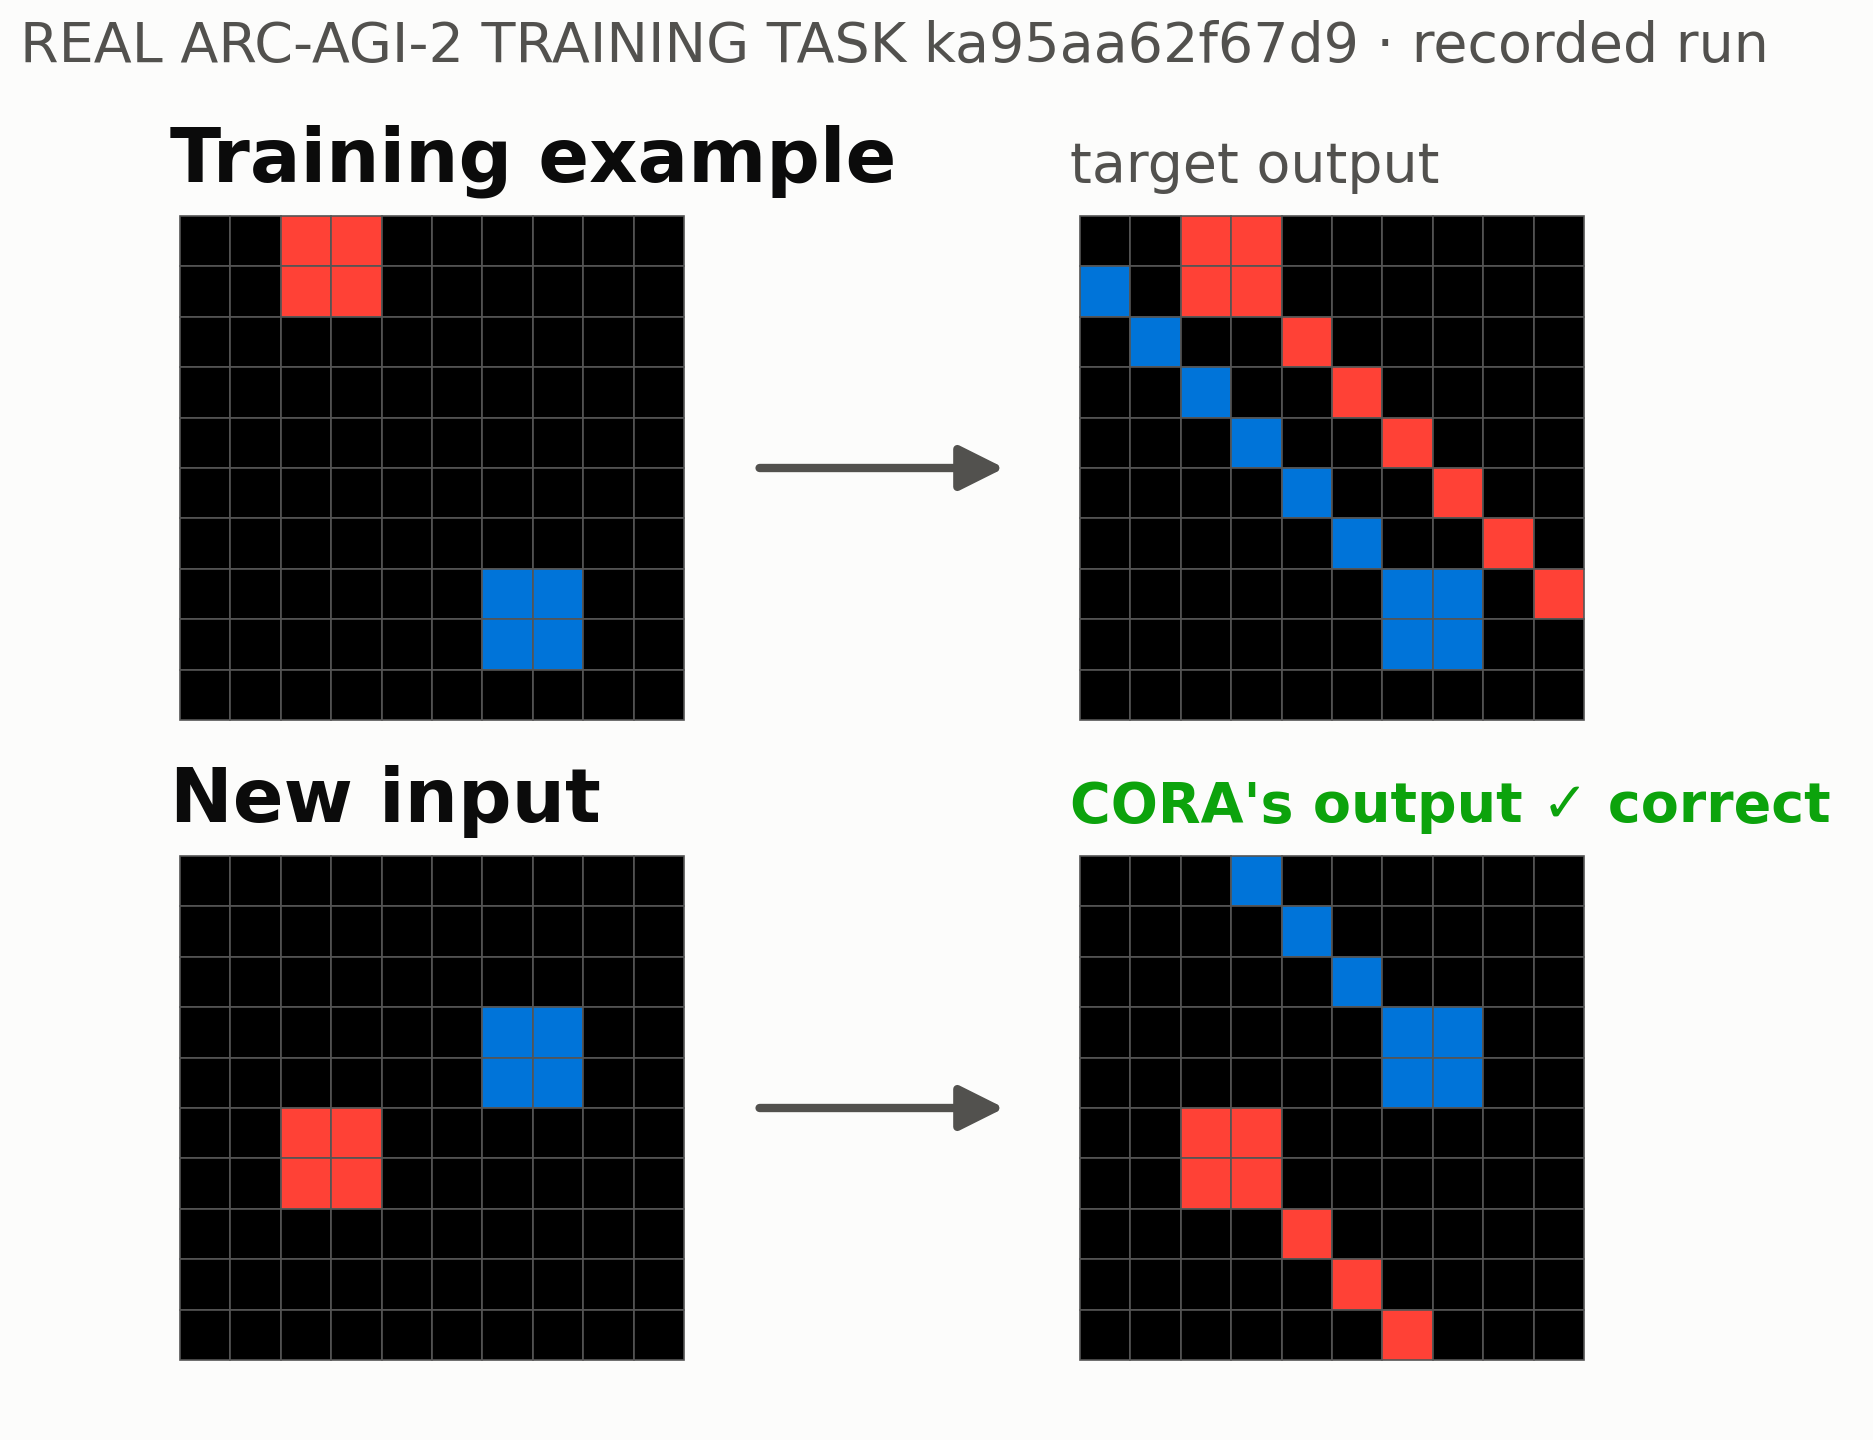
\includegraphics[width=\linewidth]{figures/fig_real_rule_ka95aa62f67d9.png}
\end{minipage}\hfill
\begin{minipage}[t]{0.46\linewidth}
\vspace{0pt}
\textbf{Figure.} Real grids from the pinned bundle (\texttt{real\_task.json} b06073a7, \texttt{real\_witness.json}
f0da3a8d): a training example with its target output, and the new input with CORA's output.
\begin{itemize}
  \item \textbf{The rule CORA constructed.} If an object's colours are \{1\}, a ray goes north-west from its centre to
        the border, otherwise south-east. In ARC colours, \textbf{blue (1) objects send a line up-left; red (2)
        objects down-right}, each in the object's own colour.
  \item \textbf{The checks.} The rule was installed reversibly in the unchanged engine and rebuilt in 3 of 3
        leave-one-out folds. The answer equals the evaluator's answer.
  \item \textbf{The comparison.} Frozen native CORA and matched extra search do not solve this task.
\end{itemize}
\end{minipage}

\textbf{Why this is not hidden-set generalization.}
\begin{itemize}
  \item The failure autopsy chose this task, in-sample, and it is an exposed public training task.
  \item A failure-blind constructor, given the same evidence, found the same rule. So the run shows that CORA can
        \emph{construct and verify} a missing rule. It does not show that diagnosing the failure \emph{caused} the
        gain (a \term{causal} claim needs a controlled comparison that the diagnosis wins).
  \item It was developed after the CORA-FHR Kaggle entry and is not part of it.
\end{itemize}

\textbf{The offline demo.} \texttt{sh docs/summit\_demo\_20261023/run\_demo.sh --real} needs Python with numpy. It is
a \emph{recorded replay}:
\begin{itemize}
  \item it prints the recorded task, native's failure, the constructed rule, the engine check and the evaluator's
        verdict;
  \item it re-executes the constructed operation as standalone code (\texttt{guard\_standalone.py}) on the test input's
        objects.
\end{itemize}
It is not a live rerun of the full engine. It was validated on 19 October (exit code 0).

%------------------------------------------------------------------------------------------------- page 6
\page{5. What the experiments taught: the 60-task audit and the 58-task negative}
\begin{minipage}[t]{0.50\linewidth}
\vspace{0pt}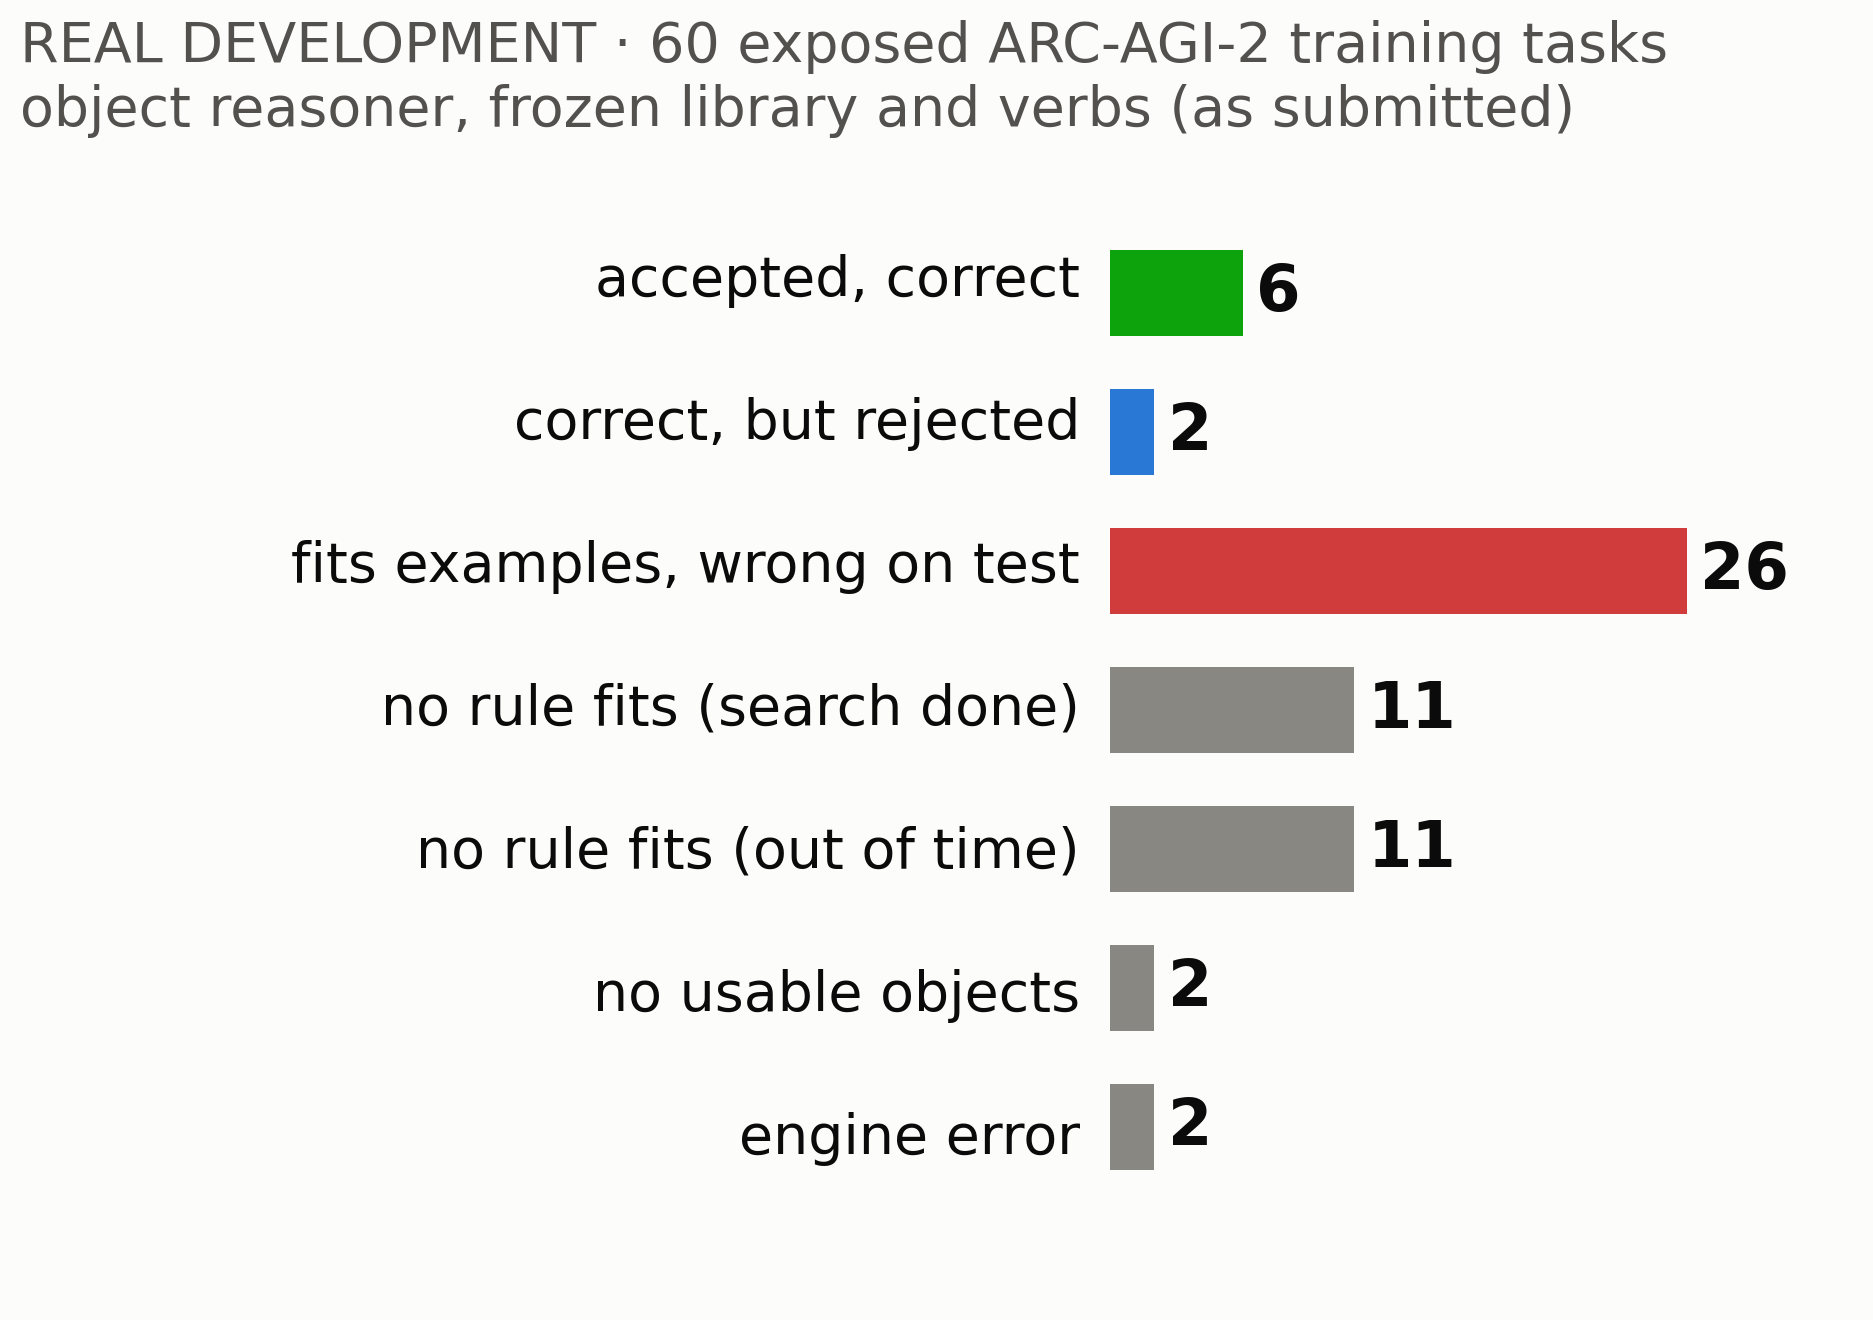
\includegraphics[width=\linewidth]{figures/fig_dev60_audit_assets.png}
\end{minipage}\hfill
\begin{minipage}[t]{0.46\linewidth}
\vspace{0pt}
\textbf{Figure: the 60-task audit.} Real data (\texttt{eval\_dev60\_native\_assets.json}, 54d8d744). It covers the
native object reasoner with its frozen library and learned verbs, as submitted, on 60 exposed ARC-AGI-2 training
tasks.
\begin{itemize}
  \item Accepted and correct: 6. Accepted and wrong: 0.
  \item 26 tasks had rules that fit every example and were all wrong on the test: \textbf{memorization}.
  \item A correct rule existed but was rejected by the check on 2 tasks; no rule fit on 22.
  \item This is one branch. The whole harness got 12 of 60 over two attempts, and the two are never mixed.
\end{itemize}
\end{minipage}

\sub{The 58-task generalization test (negative)}
\begin{itemize}
  \item \textbf{Design.} 58 separately selected, still exposed training tasks; a protocol frozen before the run.
        Arms: frozen native, matched extra search, construction from the failure record, failure-blind construction,
        shuffled evidence, and a contrast arm.
  \item \textbf{Result.} No construction arm produced a certified answer (0 of 58), with 0 wrong and 0 lost. Frozen
        native solved 1. There were no discordant pairs, so the failure record showed no advantage, and the version
        was stopped.
\end{itemize}

\sub{Why so few constructions fire: a restricted diagnostic, not a proof}
An evaluator-only (\term{oracle}) analysis, which reads the answers and is used only for diagnosis, asked one narrow
question. Can a \emph{single, unguarded, uniformly applied} G-grow expression explain the changed cells in any of
native's seven views?
\begin{itemize}
  \item For 50 of 58 tasks: no. In the sense defined here, they are \term{inexpressible} in that class.
  \item Of the other 8, 5 need colour behaviour no single such expression provides, and 3 pass the necessary checks.
\end{itemize}
This does \emph{not} show that the tasks are impossible for CORA or need entirely new semantics. Guarded, deeper or
re-segmented programs were not tested. It supports an expressivity hypothesis. Never say ``56/58 impossible''.

%------------------------------------------------------------------------------------------------- page 7
\page{6. CORA-v2: many hypotheses, ambiguity and fragile checks (poster column 3)}
\begin{center}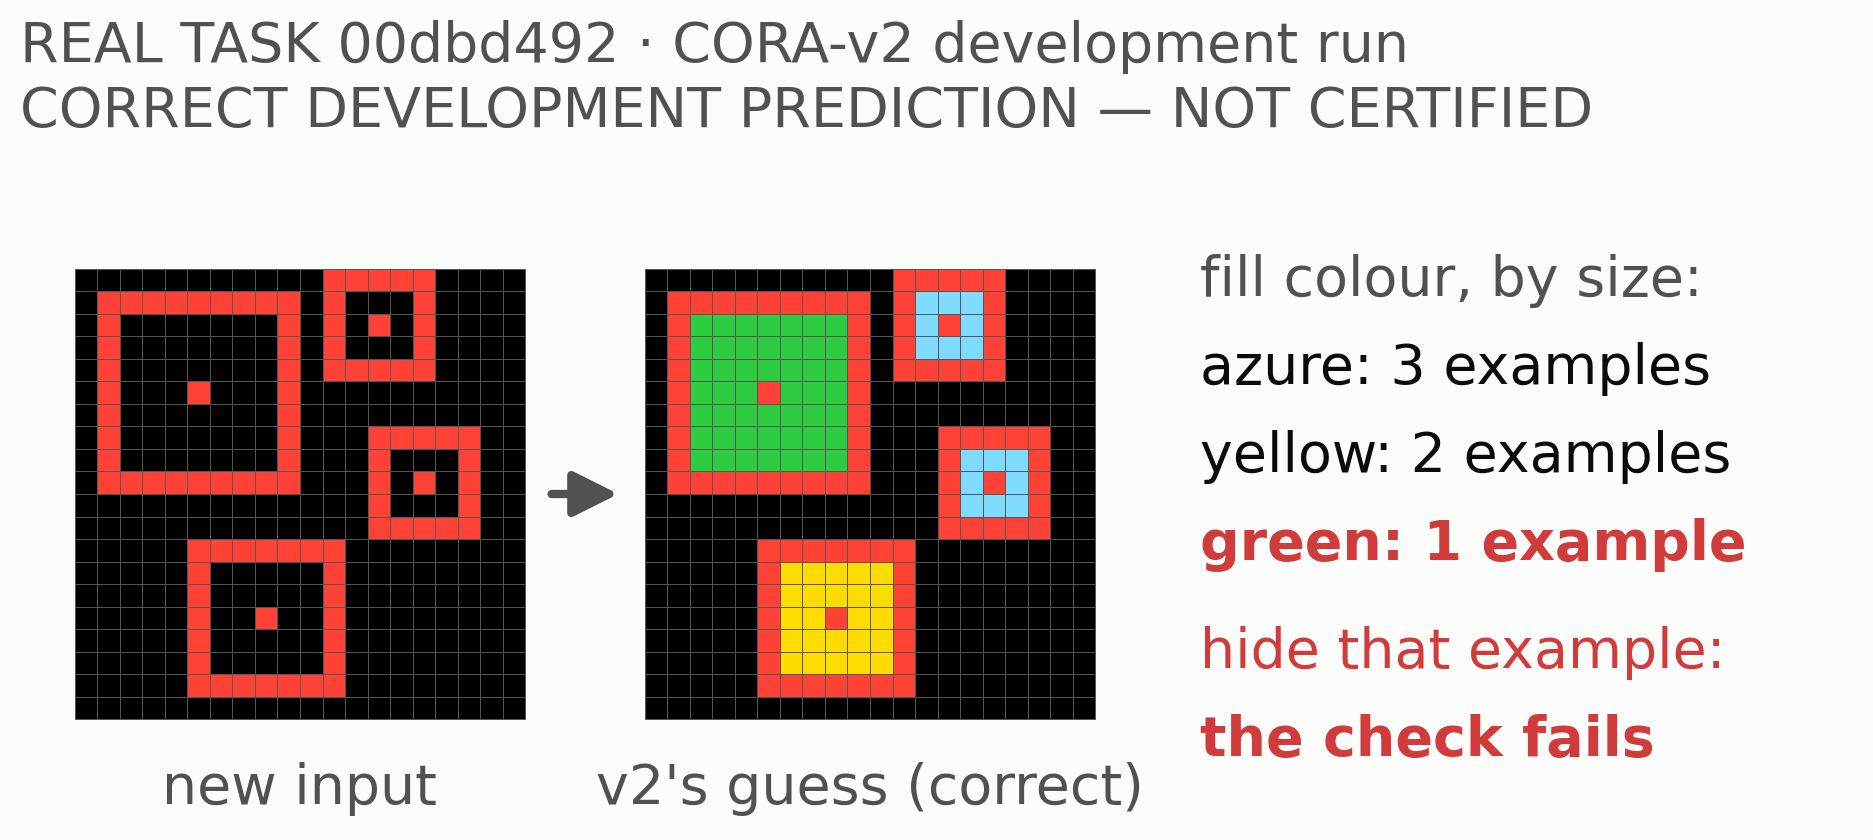
\includegraphics[width=0.62\linewidth]{figures/fig_v2_uncertified_00dbd492_poster.png}\end{center}
\textbf{Figure: task 00dbd492}, real data from the v2 engineering run.
\begin{itemize}
  \item \textbf{The guess.} v2's 1,365 consistent hypotheses all agree, and the guess is correct. Frozen native and
        matched search have no certified answer.
  \item \textbf{Why it is not certified.} The test needs the colour for the size-32 frame (green), and only one
        example shows it. With that example hidden, the rebuilt rule has no entry for size 32 and abstains: it does
        not predict wrongly.
  \item \textbf{The diagnosis.} Checks on the examples rule out ambiguity, a wrong representation and a defect. The
        cause is \emph{insufficient evidence}. A failure-blind reasoner gives the same answer.
\end{itemize}
It is an \textbf{exploratory}, uncertified prediction on an exposed task.

\sub{Engineering evidence on 118 exposed development tasks (in-sample)}
\begin{center}
\begin{tabular}{@{}lcc@{}}
\toprule
 & growth only (frozen v2) & growth + object selection \\ \midrule
certified & 0 & 0 \\
58 pool tasks: exploratory correct / wrong & 3 / 1 & 4 / 0 \\
60 dev tasks: exploratory correct / wrong & 1 / 0 & 2 / 0 \\
mean CPU per task & 20 s and 12 s & 40 s and 27 s \\ \bottomrule
\end{tabular}
\end{center}
\begin{itemize}
  \item \textbf{More rules can mean less certainty.} On 22eb0ac0, adding object selection everywhere turned a unique
        answer into a disagreement. That is a concrete reason to revise where a diagnosis asks for it, not
        everywhere.
  \item \textbf{Where whole-object operations fall short.} On 22 development tasks objects change only in part:
        \begin{itemize}
          \item native's built-in object parts fully explain 2 and partly explain 8;
          \item 7 are unexplained, often by parts that touch other objects;
          \item 5 show no partly changed object.
        \end{itemize}
        A two-stage whole-object transformation produced 0 predictions on 32 routed tasks. These are planning
        results, not accuracy.
  \item \textbf{Two attempts} (evaluator-side replay, no submission). Adding v2's exploratory guesses to native's
        recorded attempts gives:
        \begin{itemize}
          \item 58 pool tasks: 7 $\to$ 8 when filling only duplicate second attempts, 9 when always the second attempt;
          \item 60 dev tasks: 12 $\to$ 12;
          \item no answers lost.
        \end{itemize}
        This is in-sample, so not evidence for an entry.
\end{itemize}

%------------------------------------------------------------------------------------------------- page 8
\page{7. Inventing new operations: the automatic rule-language extension (Step B)}
\cue{poster column 3, ``Inventing new operations''}
\textbf{What it is.} Step B is a separate CORA Level-4 experiment, in its own repository and run. It asks whether a
system can construct genuinely new, reusable operations instead of depending only on operations a researcher
specified.
\begin{itemize}
  \item \textbf{K2.} It uses a frozen, generic, typed constructor language: a finite, closed set of type-directed
        semantic constructors, in 7 families of 19 schemas.
  \item \textbf{The run.} K2 is applied uniformly to failure clusters identified earlier, in a single run of 62
        clusters.
  \item \textbf{What it must separate.} Repairing an existing learner versus inventing a new \term{semantic
        extension}: an operation whose meaning the old language could not express.
\end{itemize}

\textbf{Status, 19 October 2026, from its counts-only administrative watcher.}
\begin{itemize}
  \item 475 of 497 K2 proposal units are done, with no errors.
  \item No completion marker and no output hash yet.
  \item No verdict on novelty or held-out transfer.
\end{itemize}

\textbf{What still has to happen.} When proposal generation finishes, the outputs are frozen and hashed before anyone
inspects them. Then come a bounded novelty check and the reserved transfer evaluation. Finishing the proposals is not
evidence of invention.

\textbf{How it relates to CORA-FHR and CORA-v2.} All three ask what to do when the current language is not enough.
\begin{itemize}
  \item FHR constructs a missing operation from a fixed growth grammar for one task.
  \item v2 compares hypotheses and diagnoses why they are not enough.
  \item Step B tests whether a generic constructor language can produce new reusable operations.
\end{itemize}
Step B's code is \textbf{not integrated} into CORA-v2 or any Kaggle entry, and none of its protected outputs were
read for this poster.

%------------------------------------------------------------------------------------------------- page 9
\page{8. What the neural baseline taught us, and what fusion would test}
\cue{poster bottom band, ``Two approaches to ARC''}
\textbf{What I reproduced.} NVARC is a published neural ARC approach. I deployed it from the public NVARC notebook
(originality audit, \texttt{records/KAGGLE\_NEURAL\_V1\_ORIGINALITY\_AUDIT\_20261014.md}).
\begin{itemize}
  \item \textbf{Unchanged:} the Qwen3-4B checkpoint, which the NVARC team pretrained on their synthetic data; their
        per-task LoRA test-time training; their decoding, candidate scoring and selection.
  \item \textbf{My six changes} were compatibility, coverage, diagnostics, provenance and robustness, not new
        algorithms.
  \item \textbf{Score.} It scored 27.64 on the official public board (Kaggle 57160429). It is a strong baseline,
        \textbf{not CORA}.
  \item \textbf{It does learn on each task:} its inference adapts the model to each puzzle's demonstrations. I did not
        invent or change that learning method.
\end{itemize}
For comparison, native CORA scored 0.00 (57144804), and CORA with rule construction 0.00 (57354496).

\textbf{What the gap means, and what it does not.} The tested neural system produces many more correct ARC predictions
than the tested symbolic system. That does not show that neural networks reason and programs cannot. It does suggest
asking what learned models could contribute \emph{inside} CORA: representation proposals, program proposals, search
guidance, uncertainty, and revision choice.

\textbf{What combining them tested, and what it did not.} A local audit filled NVARC's empty second attempts with
CORA's answers on 240 exposed stand-in tasks. It gained nothing and lost one task: a correct 1$\times$1 placeholder
\texttt{[[0]]}. That tested \emph{answer combination}. It did not test neural \emph{proposals} feeding symbolic
construction, diagnosis, revision and verification. That pipeline is untested.

\textbf{The open question.} Can learned neural representations and proposals help an executable reasoner find which
part of a hypothesis needs revision?

\textbf{What a real fusion would do} (PROPOSED: no part of it is implemented or run).
\begin{center}
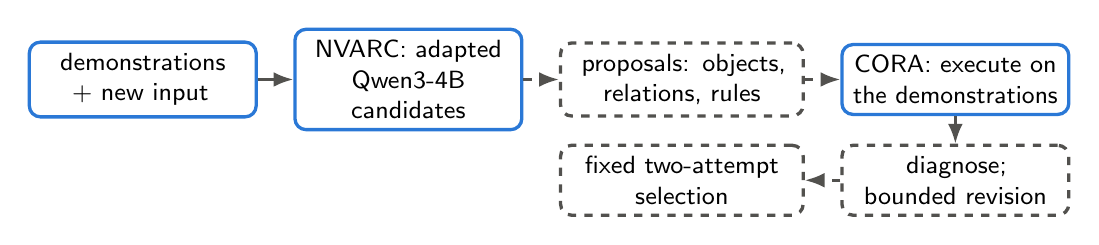
\begin{tikzpicture}[node distance=0.35cm and 0.45cm]
  \node[stage, text width=2.6cm] (d) {demonstrations + new input};
  \node[stage, right=of d, text width=2.6cm] (n) {NVARC: adapted Qwen3-4B candidates};
  \node[pstage, right=of n, text width=2.8cm] (p) {proposals: objects, relations, rules};
  \node[stage, right=of p, text width=2.6cm] (c) {CORA: execute on the demonstrations};
  \node[pstage, below=of c, text width=2.6cm] (g) {diagnose; bounded revision};
  \node[pstage, left=of g, text width=2.8cm] (s) {fixed two-attempt selection};
  \draw[flow] (d) -- (n); \draw[flow, dashed] (n) -- (p); \draw[flow, dashed] (p) -- (c); \draw[flow, dashed] (c) -- (g);
  \draw[flow, dashed] (g) -- (s);
\end{tikzpicture}
\end{center}
\begin{itemize}
  \item \textbf{Verification.} A neural candidate grid, or a confident score, is a proposal, not a verification. CORA
        would accept a proposed rule only if it executes and reproduces every demonstration, and certify it only under
        the unchanged checks.
  \item \textbf{Fallback.} If no proposal helps, the output stays NVARC's unchanged.
  \item \textbf{Status.} The saved NVARC run kept only its final answers, so a fusion first needs an instrumented run
        that records the candidates and their scores (\texttt{records/CORA\_QWEN\_FUSION\_FEASIBILITY\_20261019.md}).
\end{itemize}

\textbf{A first experiment after the summit} (a design idea, not authorized, not run). It would use exposed engineering
tasks, with four conditions:
\begin{itemize}
  \item CORA-v2;
  \item CORA-v2 with matched extra symbolic search;
  \item CORA-v2 with neural proposals (objects, parts, candidate rules);
  \item neural proposals chosen by observable diagnostic evidence.
\end{itemize}
Rules for the experiment:
\begin{itemize}
  \item measure \emph{candidate coverage} (is a correct hypothesis proposed?) separately from correct final
        predictions;
  \item neural outputs stay untrusted proposals until verified;
  \item if the neural model is adapted to a task's demonstrations, leave-one-out checks must repeat that adaptation
        without the held-out demonstration.
\end{itemize}
Modern LLMs can reason, use tools and check their work, and I do not claim otherwise. CORA asks a narrower question
about inspectable, reversible, component-level revision.

%------------------------------------------------------------------------------------------------- page 10
\page{9. Where this sits in prior work}
\textbf{The general loop of failing, revising and checking is not new.} The possible difference is narrow and testable.
\begin{itemize}
  \item \textbf{Popper} (Cropper and Morel, \emph{Learning programs by learning from failures}, Machine Learning,
        2021). Inductive logic programming that turns failed hypotheses into constraints that prune the search. It
        overlaps with using failure to guide search. CORA additionally asks which \emph{component} (objects, rule
        language, evidence) to revise, in grid reasoning.
  \item \textbf{DreamCoder} (Ellis et al., PLDI 2021). Wake--sleep library learning that grows reusable abstractions
        and a neural search guide. It overlaps with growing a rule language, which is closest to Step B.
  \item \textbf{LILO} (Grand et al., ICLR 2024). LLM-guided program synthesis with library compression and
        auto-documentation. It overlaps with LLM-proposed programs and abstractions.
  \item \textbf{Model Discovery Agent} (Murphy, 2026). LLM-assisted Bayesian experiment design for data-efficient
        discovery of mechanistic models: recognizing model inadequacy, proposing new models, choosing experiments. It
        is closest to the scientific framing.
\end{itemize}
\textbf{The narrow claim to be tested.} A diagnosis-driven choice of \emph{which component to revise} beats, under
matched compute and matched evidence:
\begin{itemize}
  \item a strong failure-blind choice;
  \item applying every revision;
  \item a shuffled diagnosis.
\end{itemize}
It must also add correct predictions on tasks the system was not developed on. None of these systems is said to be
unable to do this.

%------------------------------------------------------------------------------------------------- page 11
\page{10. How to test whether diagnosis helps}
\textbf{What a convincing test needs.}
\begin{itemize}
  \item \textbf{A fresh cohort.} Tasks not used in development, chosen by a rule declared beforehand.
  \item \textbf{Strong controls.}
        \begin{itemize}
          \item frozen native;
          \item matched extra search;
          \item a strong failure-blind revision;
          \item every revision applied everywhere;
          \item the same at matched compute;
          \item a shuffled diagnosis.
        \end{itemize}
  \item \textbf{Harm counted.} Wrong certified answers and lost answers are counted, not only gains.
  \item \textbf{Separate tiers.} Certified and exploratory answers are reported separately.
  \item \textbf{A blind evaluator} that reads answers only after every prediction is frozen.
  \item \textbf{A pre-registered decision rule}, applied without retuning on the evaluated tasks.
\end{itemize}
A \term{prospective} test is one whose design and cohort are fixed before any result is seen.

\textbf{Phase 2a status: RUNNING, RESULT PENDING.}
\begin{itemize}
  \item \textbf{Cohort.} 40 public training tasks.
        \begin{itemize}
          \item They were selected by a declared rule and are independent of all v2 development.
          \item A single authorized, metadata-only check excluded Step B's protected splits: 44 of 100 candidates were
                eligible, and the first 40 were used.
          \item They are reused public tasks, so a result is a development evaluation, not a blind prospective test
                or an unseen-task score.
        \end{itemize}
  \item \textbf{Arms.} Frozen native (A), matched extra search (B), and the frozen growth-only v2 (V).
  \item \textbf{GO rule.}
        \begin{itemize}
          \item complete coverage and valid hashes;
          \item zero wrong certified v2 answers;
          \item at least 2 tasks where v2 is right and A and B are not.
        \end{itemize}
  \item \textbf{Reporting.} The result will be added here and to the ledger only after its integrity checks.
\end{itemize}

\textbf{If GO, Phase 2b.} It would test the causal question: does the diagnosis choose better revisions than applying
everything, at matched compute, or a shuffled diagnosis? It needs a new eligible cohort and approval.

\textbf{If NO-GO.} The version is closed. The next step would be one small, evidence-based change: part-aware or
relational object parts, chosen from the 22-task characterization on page 7.

%------------------------------------------------------------------------------------------------- page 12
\page{11. Science next, and how to reproduce everything}
\textbf{Plausible next domains.} \textbf{FUTURE, NOT TESTED}: no biological transfer or mechanism is claimed. What
might transfer is the diagnosis-and-revision policy. The operations, evidence and validators must be specific to
each domain.
\begin{itemize}
  \item \textbf{Protein conformational ensembles.} Is a structural hypothesis wrong, or is the ensemble
        representation too coarse?
  \item \textbf{Single-cell and other omics.} Is an effect a shift in average, a change in spread, or a change in the
        mixture of cell states? The level at which you infer (cells or donors) matters.
  \item \textbf{Maize lesion-mimic phenotyping.} Image geometry and topology tell you where and how lesions form,
        not which pathway is involved. Inferring a candidate pathway would need independent molecular or
        perturbation evidence.
\end{itemize}
Examples, data and wording are subject to Pierce's and Chris's input.

\sub{Reproducing what you see}
\begin{itemize}
  \item \textbf{Poster figures.} \texttt{python scripts/summit\_visual\_figures.py} writes \texttt{figures/*.png} and
        \texttt{POSTER\_FIGURE\_PROVENANCE.json}. It stops if any pinned input's sha256 differs.
  \item \textbf{Poster PDF.} From \texttt{docs/summit\_20261023\_reframe/}, run \texttt{SOURCE\_DATE\_EPOCH=1791763200
        FORCE\_SOURCE\_DATE=1 pdflatex poster\_visual\_final\_review.tex}.
  \item \textbf{Editable PowerPoint.} \texttt{python scripts/poster\_visual\_to\_pptx.py}.
  \item \textbf{Demos} (offline; Python with numpy), both validated 19 October:
        \begin{itemize}
          \item \texttt{sh docs/summit\_demo\_20261023/run\_demo.sh} replays the synthetic witness;
          \item adding \texttt{--real} replays the real ka95aa62f67d9 witness.
        \end{itemize}
        Each replays the recorded run and re-executes the constructed operation standalone.
  \item \textbf{Records.}
        \begin{itemize}
          \item ledger: \texttt{records/CORA\_SUMMIT\_CLAIM\_LEDGER\_20261017.md};
          \item v2: \texttt{records/CORA\_REASONING\_V2\_*.md};
          \item rule construction: \texttt{records/CORA\_FHR\_*.md}.
        \end{itemize}
\end{itemize}

\textbf{Credits and disclosure.} The research question was shaped in discussions with Toni Kazic. Authorship and
credits are pending review by Toni, Chris and Pierce. AI coding assistance was used for parts of the implementation
and documentation; the research, decisions and claims are the author's.
\end{document}
